\section{Generative Adversarial Networks}

In 2014, Ian Goodfellow invented Generative Adversarial Networks (GANs). The concept is rather simple, as it consists of two competing networks. The first network is called a Generator and creates new images based on an input image. Here, for consistency, the images generated by the Generator will be denoted as generated images. The second network is the Discriminator, which tries to distinguish between the generated image (predicted image) and the real image (ground truth) \cite{goodfellow2014generative}.
As a consequence of training both networks alternately, the generated images eventually become indistinguishable from the real images. It is nothing more than a two-player min-max game, a famous problem in game theory. GAN was initially proposed in the formulation form as:
\begin{equation}
	\centering
	\begin{aligned}
		\min_{G} \max_{D} V(D, G) &= \mathbb{E}_{x \sim p_{data}(x)} \left[ \log D(x) \right] \\
		&+ \mathbb{E}_{z \sim p_{z}(z)} \left[ \log \left( 1-D(G(z)) \right) \right]
	\end{aligned}
	\label{eq:Basic_GAN}
\end{equation}
here, $V(D, G)$ is the value function of the min-max game. 

The goal is now to learn the distribution of the Generator $p_g$ over the data $x$. We have input noise variables $p_z(z)$, as well as the two perceptrons $G(z; \theta_g)$ and $D(x; \theta_d)$ with parameters $\theta_i$. $G$ represents a differential function that maps from $z$ to the data space $x$, while $D(x)$ represents the probability that $x$ is from the real data \cite{goodfellow2014generative}. The problem can be reformulated as: 
\begin{equation}
	\centering
	\begin{aligned}
		\max_{D} V(G, D) &= \mathbb{E}_{x \sim p_{data}} \left[ \log D^{*}_{G}(x) \right] \\ 
		&+ \mathbb{E}_{x \sim p_{g}} \left[ \log \left( 1 - D^{*}_{G}(x) \right) \right]
	\end{aligned}
	\label{eq:GAN_reformulated}
\end{equation}
where $D^{*}_{G}$ denotes the optimum of the Discriminator for a given fixed Generator and is expressed as
\begin{equation}
	\centering
	D^*_G(x) = \frac{p_{data}(x)}{p_{data}(x) + p_g(g)}
	\label{eq:Disc_optimum}
\end{equation}
It can now be shown that the global optimum of equation (\ref{eq:GAN_reformulated}) is reached if and only if $p_g = p_{data}$. Furthermore, if both $G$ and $D$ are allowed to reach their optima, $p_g$ converges to $p_{data}$. A more detailed discussion of the problem, including proofs, can be found in \cite{goodfellow2014generative}.
\begin{figure}
	\centering
	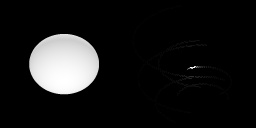
\includegraphics[width=\linewidth]{fig/ellipsoid_0.jpg}
	\caption{Merged image, which includes the original and the sparsely sampled Fourier plane. It is exactly what the GAN receives. }
	\label{fig:GANinput}
\end{figure}
\begin{figure}
	\centering
	\begin{subfigure}{\linewidth}
		\centering
		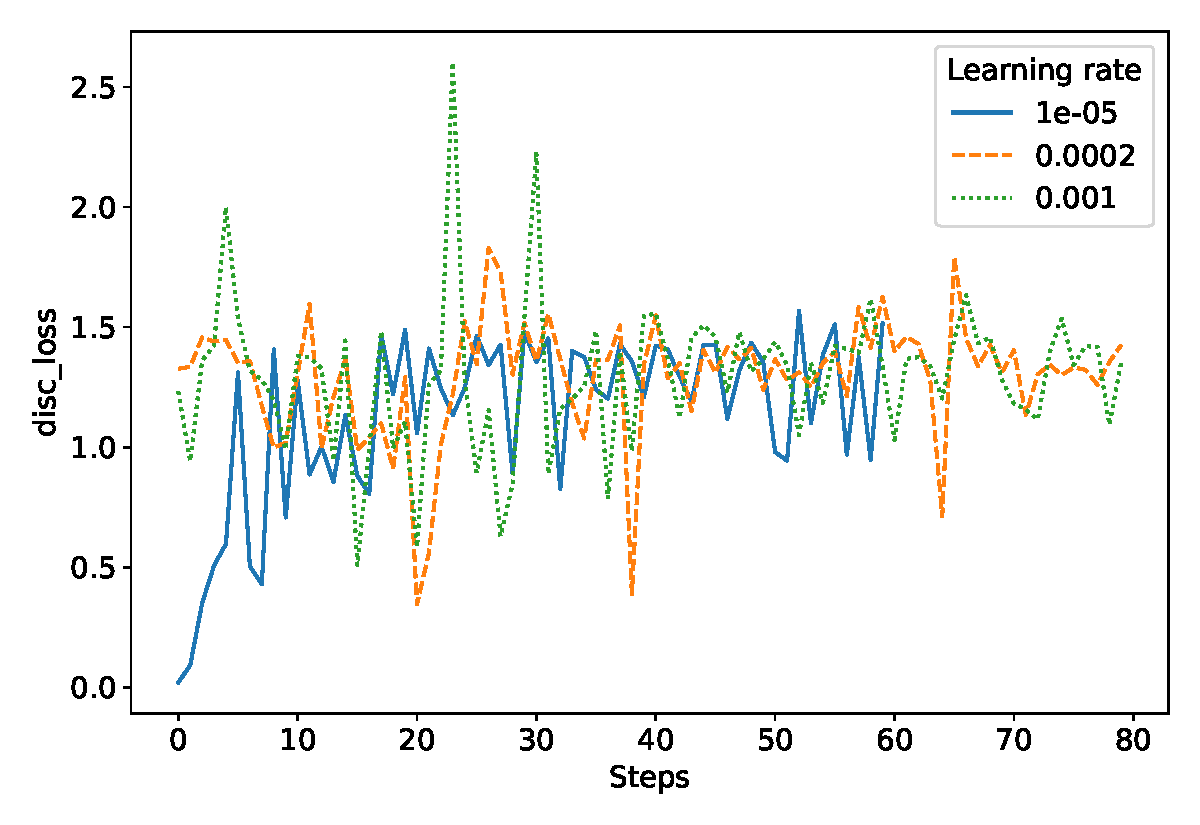
\includegraphics[width=\textwidth]{fig/analysis/Plot_learning_rate_disc_loss.pdf}
		\caption{Discriminator loss for three different learning rates. }
		\label{fig:Plot_learning_rate_discloss}
	\end{subfigure}\hfill
	\begin{subfigure}{\linewidth}
		\centering
		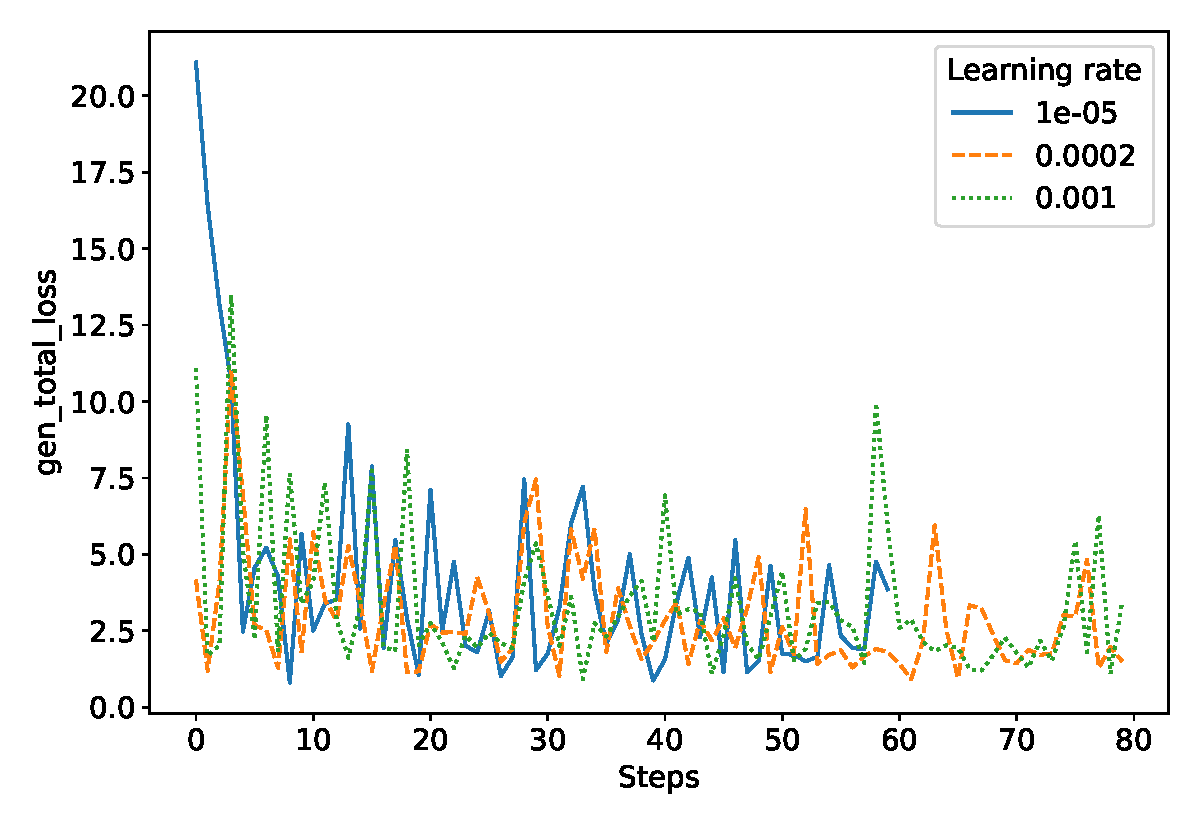
\includegraphics[width=\textwidth]{fig/analysis/Plot_learning_rate_gen_total_loss.pdf}
		\caption{Total generator loss for different learning rates (eqn. (\ref{eq:total_gen_loss})).}
		\label{fig:Plot_learning_rate_genloss}
	\end{subfigure}\hfill
	\caption{Generator and Discriminator losses for three different learning rates. The upper figure shows the total Discriminator loss, and the lower figure shows the total generator loss. There is no significant difference, but the highest learning rate might be prone to outliers. }
	\label{fig:Plot_learning_rate_loss}
\end{figure}
\begin{figure}
	\centering
	\begin{subfigure}{\linewidth}
		\centering
		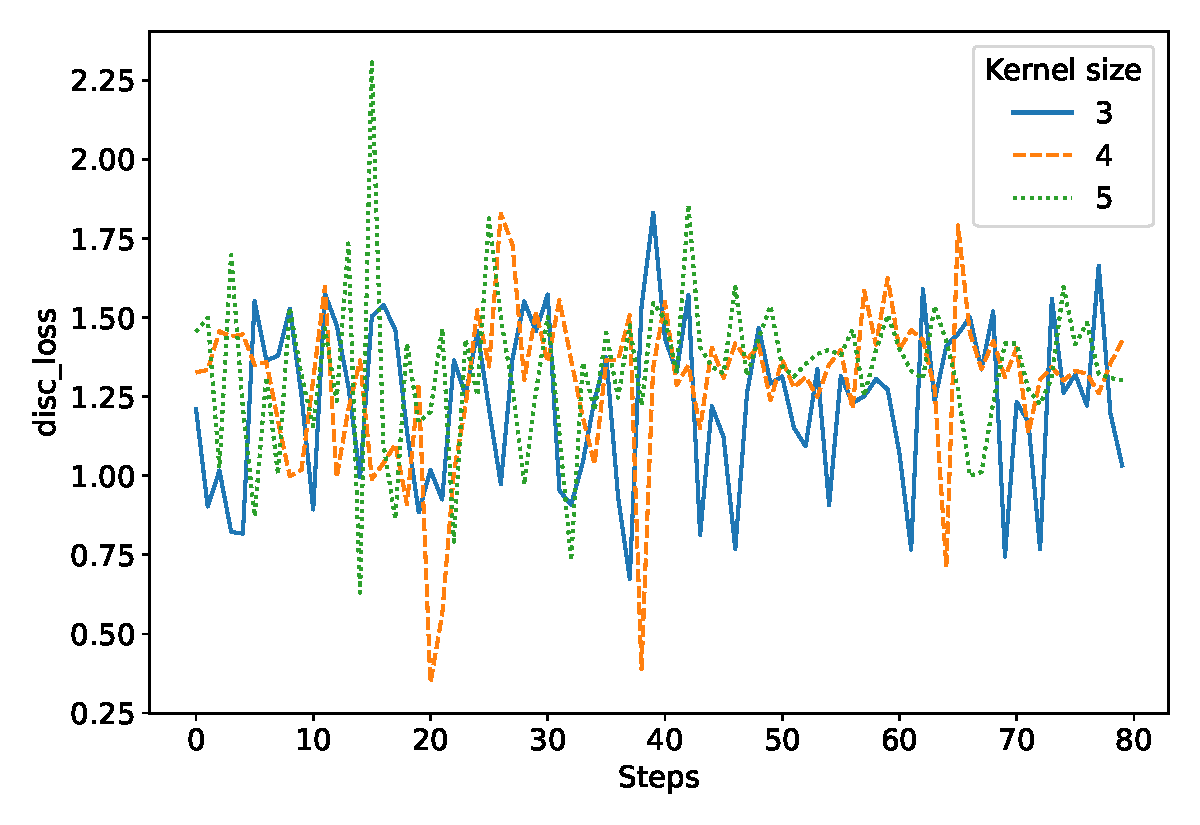
\includegraphics[width=\textwidth]{fig/analysis/Plot_Kernel_size_disc_loss.pdf}
		\caption{Discriminator loss for three different kernel sizes. }
		\label{fig:Plot_kernel_size_discloss}
	\end{subfigure}\hfill
	\begin{subfigure}{\linewidth}
		\centering
		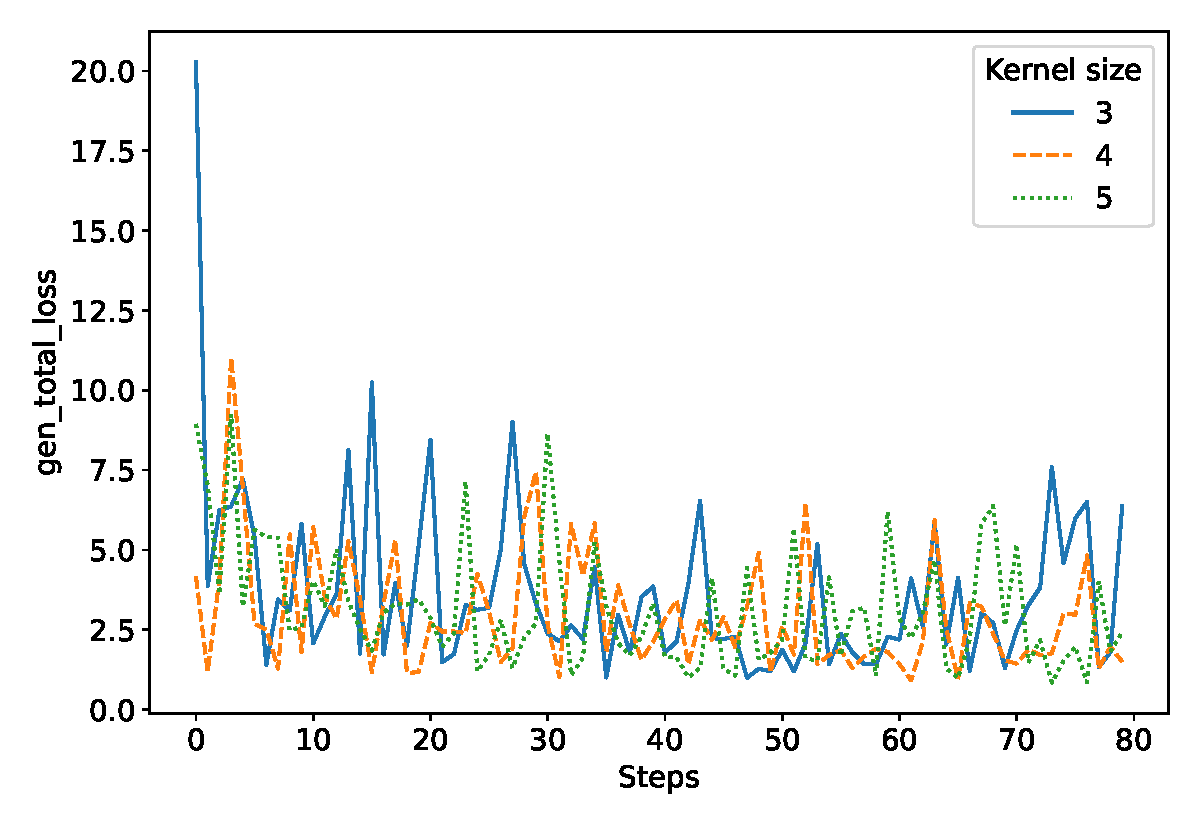
\includegraphics[width=\textwidth]{fig/analysis/Plot_Kernel_size_gen_total_loss.pdf}
		\caption{Total generator loss for three different kernel sizes.}
		\label{fig:Plot_kernel_size_genloss}
	\end{subfigure}\hfill
	\caption{Generator and Discriminator losses for three different kernel sizes in the convolutional layers. Here, the smallest kernel size has many outliers, while the largest kernel size seems to be the most stable.}
	\label{fig:Plot_kernel_size_loss}
\end{figure}
\begin{figure*}
	\centering
	\begin{subfigure}{0.5\linewidth}
		\centering
		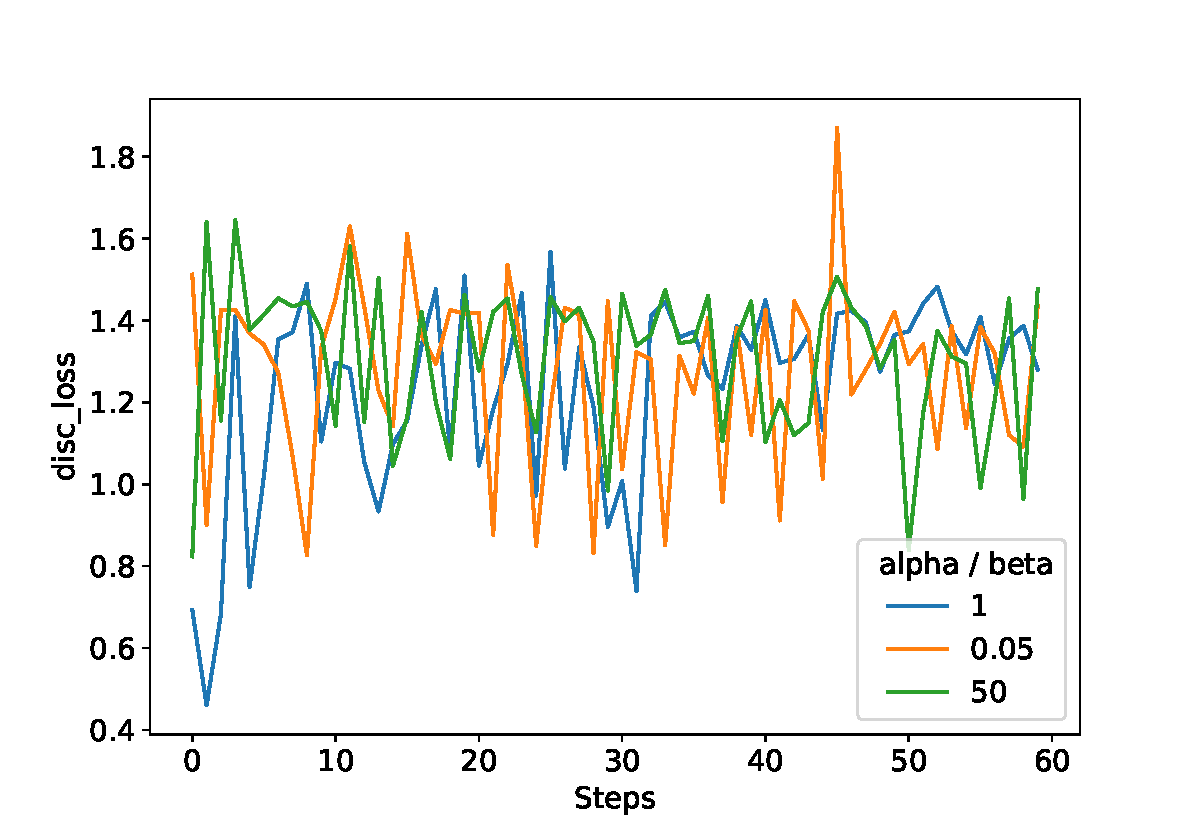
\includegraphics[width=\textwidth]{fig/analysis/Plot_noise_factor_disc_loss.pdf}
		\caption{Discriminator loss for different noise percentages.}
		\label{fig:Plot_noise_discloss}
	\end{subfigure}\hfill
	\begin{subfigure}{0.5\linewidth}
		\centering
		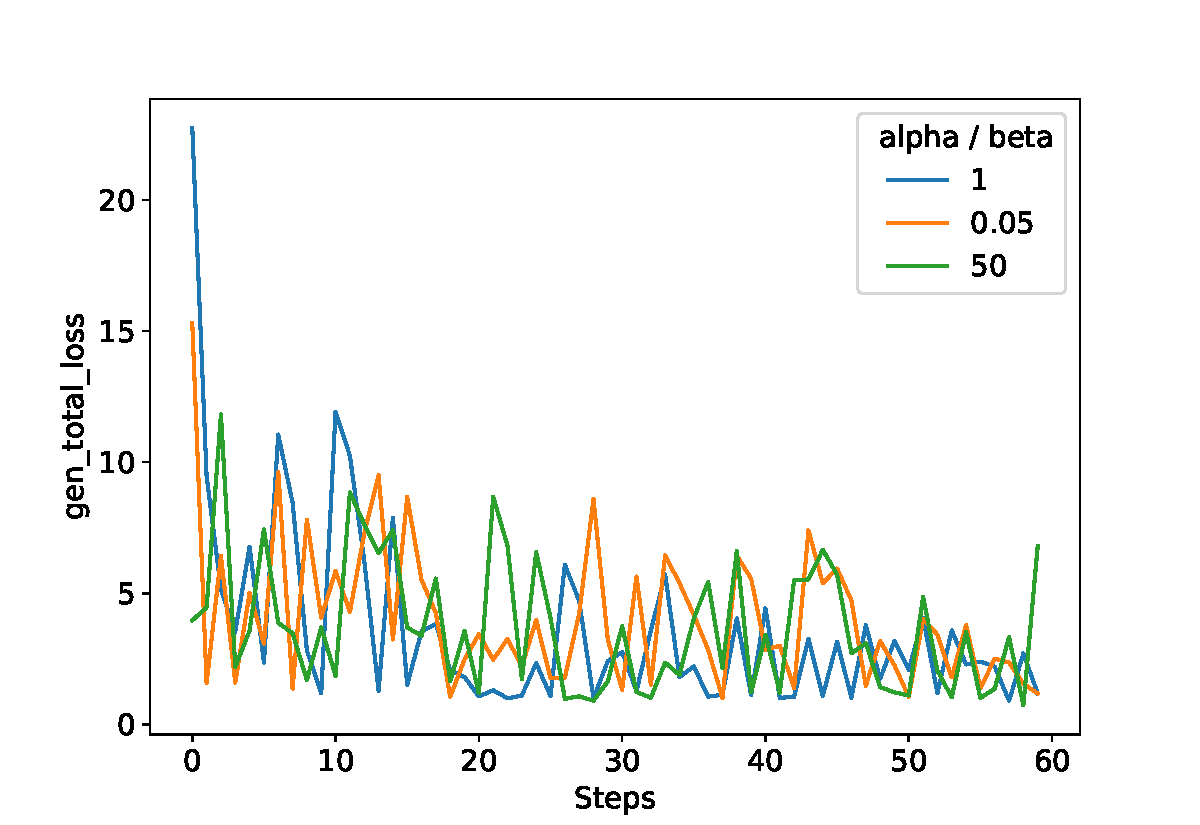
\includegraphics[width=\textwidth]{fig/analysis/Plot_noise_factor_gen_total_loss.pdf}
		\caption{Generator losses for different noise percentages.}
		\label{fig:Plot_noise_genloss}
	\end{subfigure}\hfill
	\caption{Effect of the Salt and Pepper noise introduced in the images. Different ratios between $\alpha$ and $\beta$ are shown. There is no significant effect. Please note that these results are from training on 64-pixel images.}
	\label{fig:Plot_noise_loss}
\end{figure*}
\begin{figure*}
	\centering
	\begin{subfigure}{0.5\linewidth}
		\centering
		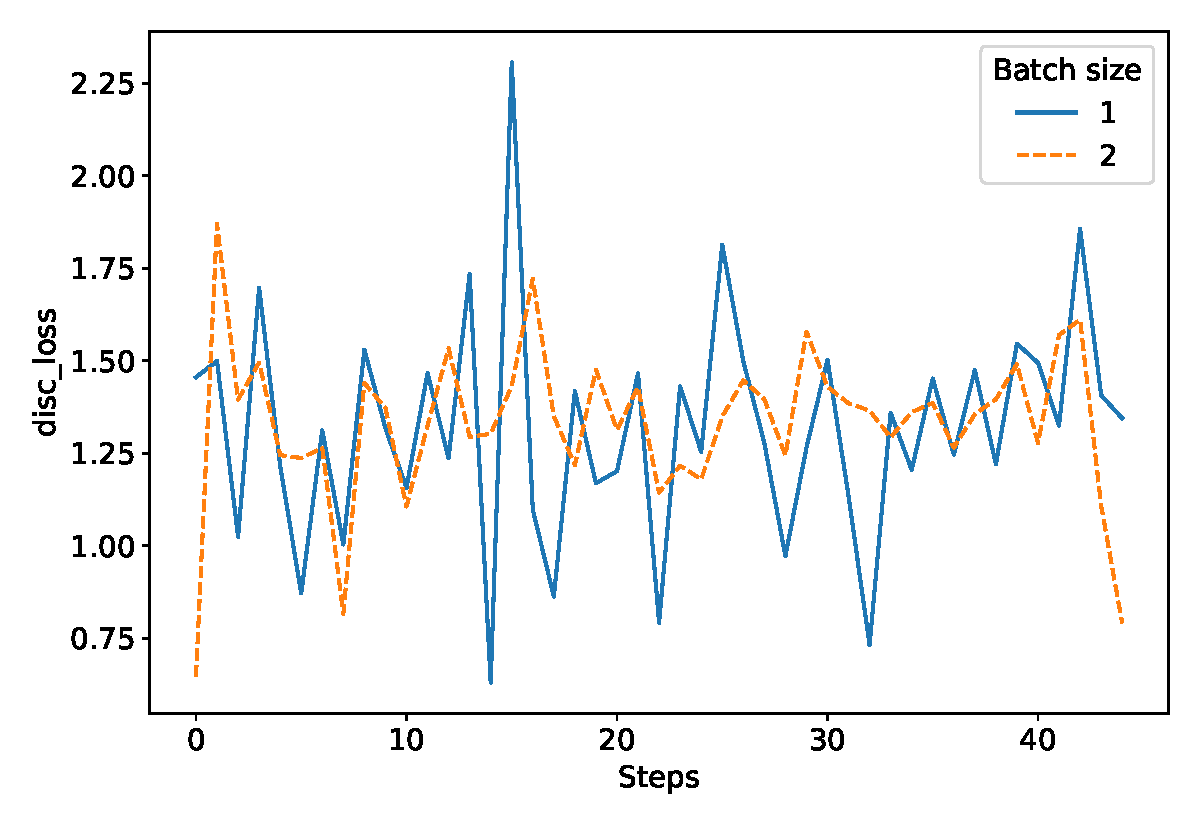
\includegraphics[width=\textwidth]{fig/analysis/Plot_Batchsize_disc_loss.pdf}
		\caption{Discriminator loss for different batch sizes.}
		\label{fig:Plot_batchsize_discloss}
	\end{subfigure}\hfill
	\begin{subfigure}{0.5\linewidth}
		\centering
		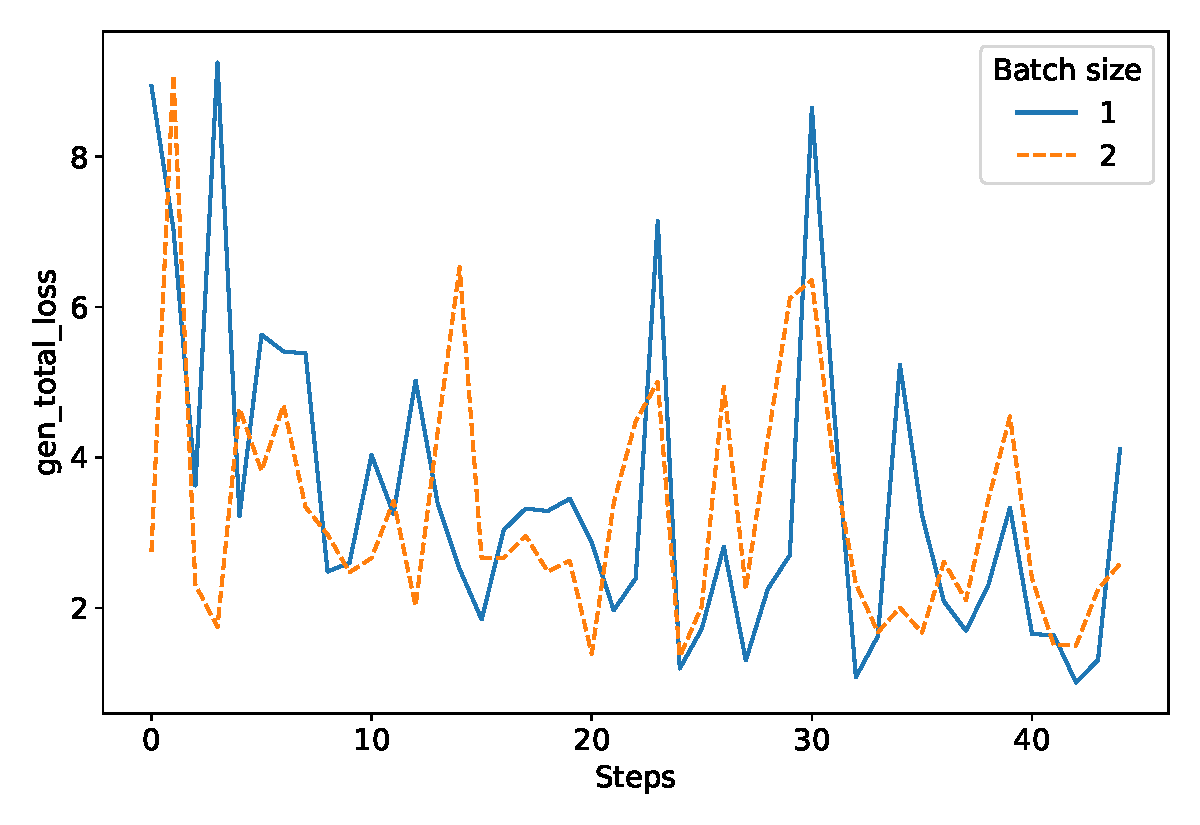
\includegraphics[width=\textwidth]{fig/analysis/Plot_Batchsize_gen_total_loss.pdf}
		\caption{Generator losses for different batch sizes.}
		\label{fig:Plot_batchsize_genloss}
	\end{subfigure}\hfill
	\caption{Loss functions for two different batch sizes. Large batch sizes seem to be more robust, but they also increase training time significantly. }
	\label{fig:Plot_batchsize_loss}
\end{figure*}
\begin{figure*}
	\centering
	\begin{subfigure}{0.5\linewidth}
		\centering
		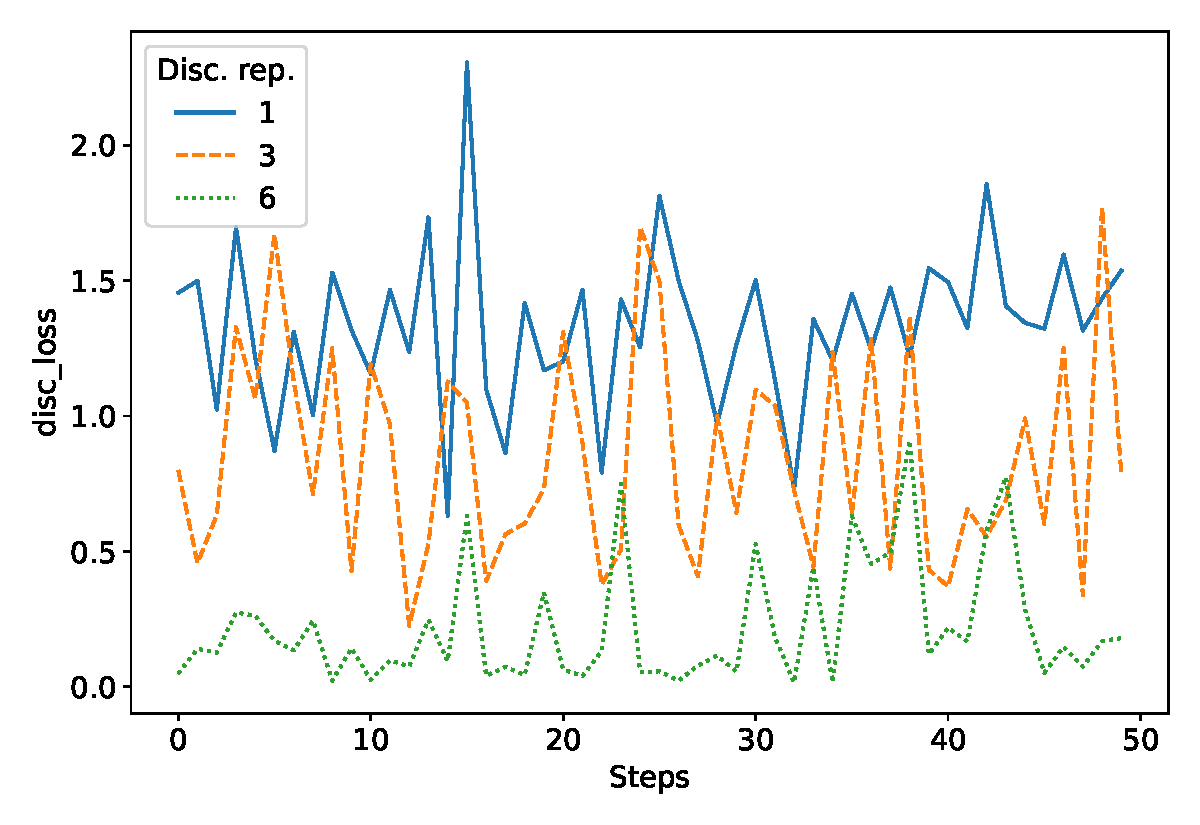
\includegraphics[width=\textwidth]{fig/analysis/Plot_Disc_rep_disc_loss.pdf}
		\caption{Discriminator loss for different Discriminator training.}
		\label{fig:Plot_discrep_discloss}
	\end{subfigure}\hfill
	\begin{subfigure}{0.5\linewidth}
		\centering
		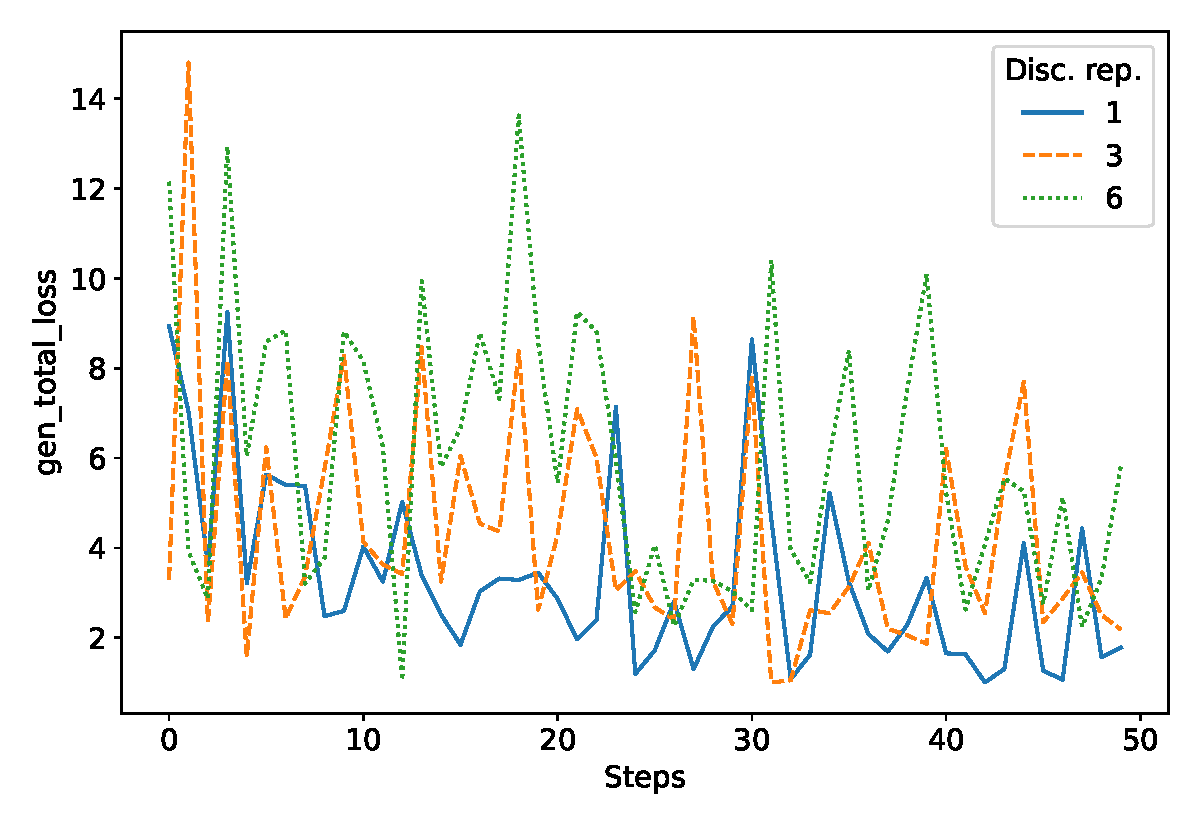
\includegraphics[width=\textwidth]{fig/analysis/Plot_Disc_rep_gen_total_loss.pdf}
		\caption{Generator losses for different Discriminator training.}
		\label{fig:Plot_discrep_genloss}
	\end{subfigure}\hfill
	\caption{The amount of Discriminator training has a high impact on the Discriminator score. The Discriminator repetition indicates the factor by which the Discriminator is trained more with respect to the Generator.}
	\label{fig:Plot_discrep_loss}
\end{figure*}
\begin{figure*}
	\centering
	\begin{subfigure}{0.5\linewidth}
		\centering
		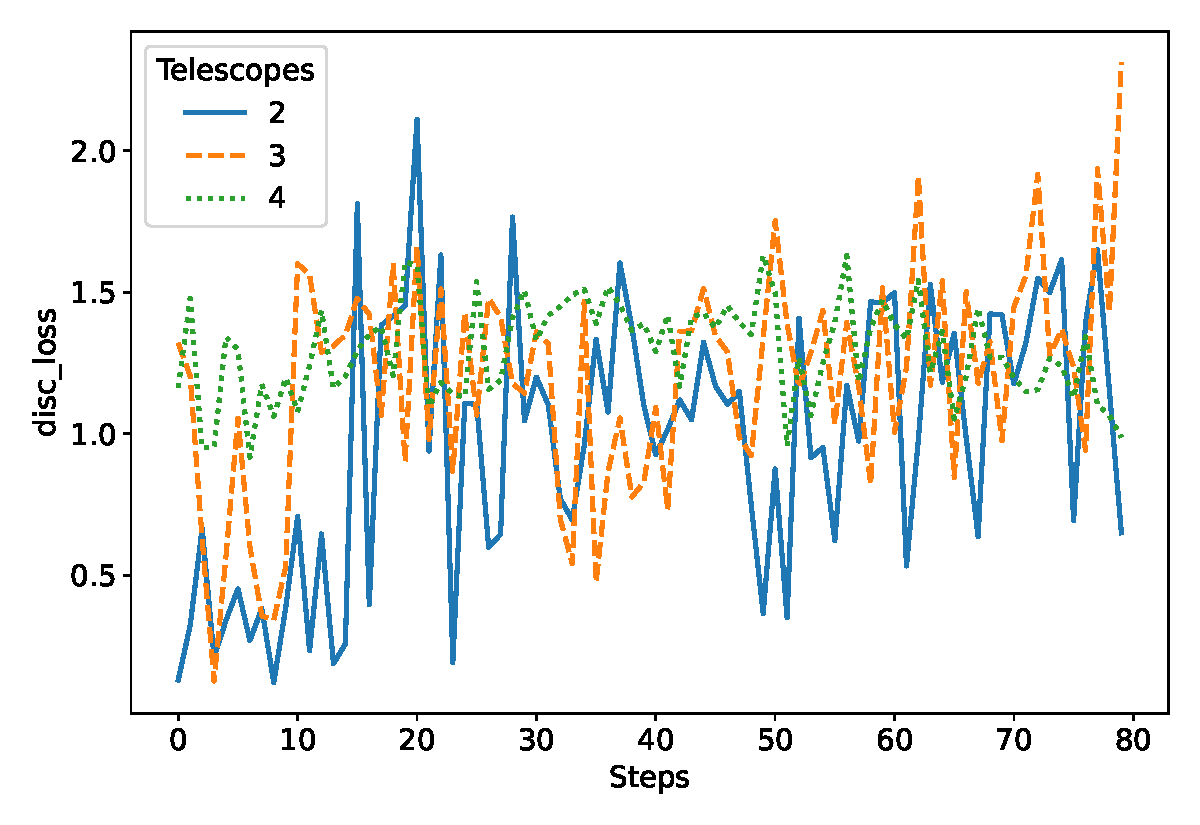
\includegraphics[width=\textwidth]{fig/analysis/Plot_N_telescopes_disc_loss.pdf}
		\caption{Discriminator loss for different amounts of telescopes.}
		\label{fig:Plot_telescopes_discloss}
	\end{subfigure}\hfill
	\begin{subfigure}{0.5\linewidth}
		\centering
		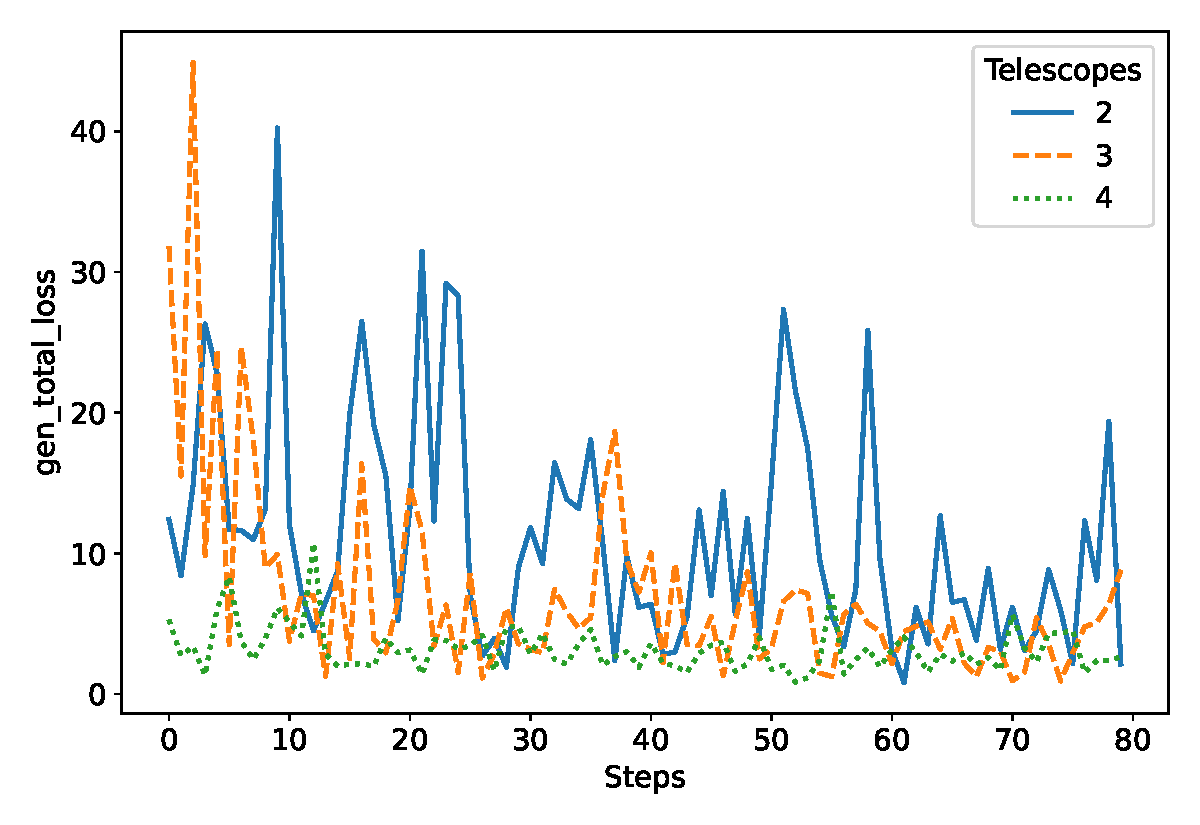
\includegraphics[width=\textwidth]{fig/analysis/Plot_N_telescopes_gen_total_loss.pdf}
		\caption{Generator loss for different amount of telescopes.}
		\label{fig:Plot_telescopes_genloss}
	\end{subfigure}\hfill
	\caption{The number of telescopes has a very impact on the model performance. If there are only two telescopes (1 baseline), both Discriminator and Generator are not trained smoothly: One gains a big advantage over the other. The result of four telescopes (6 baselines) is a lot better because the loss functions change only slightly with increasing steps.}
	\label{fig:Plot_telescopes_loss}
\end{figure*}
Later, GAN extended its version to a conditional model \cite{mirza2014conditional}. In this case, both Generator and Discriminator receive extra information $y$, such that the value function of the conditional GAN (cGAN) is expressed as:
\begin{equation}
	\centering
	\begin{aligned}
		V(D, G) &= \mathbb{E}_{x \sim p_{data}(x)} \left[ \log D(x|y) \right] \\
		&+ \mathbb{E}_{z \sim p_{z}(z)} \left[ \log \left( 1-D(G(z|y) \right) \right]
	\end{aligned}
	\label{eq:conditional_GAN}
\end{equation}

Furthermore, \cite{isola2017image} observed that combining the cGAN given in equation \ref{eq:conditional_GAN} with the traditional L1-loss improves results, as the Generator tries to be close to the ground truth. Hence, the function that is minimized as:
\begin{equation}
	\centering
	L_{tot} = \arg \min_{G} \max_{D} V(D, G) + \lambda \cdot L_1(G)
	\label{eq:total_gen_loss}
\end{equation}
where $\lambda$ = 100 and $L_1(G)$ is given as
\begin{equation}
	\centering
	L_1(G) = \mathbb{E}_{x,y,z} \left[ ||{y - G(x,z)}||_1 \right]
	\label{eq:l1_loss}
\end{equation}

This type of network is shown to be very robust, as it has been applied to several problems. Examples include creating colored images from grayscale images based on architectural labels, changing from day to night in different pictures, and predicting a map based on satellite data. A longer list of applications is given in \cite{isola2017image}. 

\subsection{Generator}
As discussed above, in a GAN, the Generator is responsible for generating fake data; here, the generated images look like real images of a fast-rotating star. The Generator used in this paper is a common U-Net convolutional network \cite{ronneberger2015u}, where the spatial dimension of the image is reduced first using downsampling and then enhanced using upsampling, making it U-shape. The downsampling process typically consists of convolutional layers followed by a strides operation to skip some pixels of the image. Here, the filter is skipping 2 pixels at a time of operation. A leaky version of a Rectified Linear Unit is used to activate the neuron in convolutional layers of the downsampling process.

In contrast, only the Rectified Linear Unit is used to activate the neuron in the upsampling process. The upsampling process also consists of convolutional layers followed by strides = 2 operations to scale up the image for high resolution. However, there is an introduced dropout layer at the beginning of upsampling to avoid over-fitting of the model by the Generator \cite{isola2017image}.

After creating images, the Generator tries to fool the Discriminator into thinking that the generated image is similar to the real image. The level of making fools to Discriminator is called GAN loss. If the Discriminator does not distinguish between the input image and the real image (i.e., the GAN loss is minimum), the Generator stops creating images, and it is trained. However, if the generated image fails to fool the Discriminator, the Generator will again create an image to compare it with the real image. There is another loss calculated by the Generator, which is called L1 loss. It is defined based on the mean absolute error between the pixels of the real image and the generated image. The Generator tries to minimize L1 loss while taking care of GAN loss. The balance between GAN loss and L1 loss allows the Generator to generate realistic yet accurate images.

\subsection{Discriminator}
As discussed before, the Discriminator has the job of classifying the input image by the Generator as real or fake. The Discriminator takes a real image from the data set, also called the target image for the Generator. It tries to train the Generator to create a perfect image while giving feedback based on the input image. Here, the Discriminator that has been taken is PatchGAN \cite{isola2017image}, which does not work globally but rather classifies single patches as real or fake, so it outputs a grid of predictions instead of a single value. 

The model architecture of the Discriminator follows the initializer along with inputs (input images and real images). After adding Salt-and-Pepper noise to the input image, PatchGAN focuses on reducing the spatial dimensions of images to extract features, making the model focus on smaller regions of the image. In this process, a leaky version of a Rectified Linear Unit is introduced to convolutional layers as done in the Generator. Later, zero padding adds rows and columns of zeros around the images to prevent loss of spatial information during convolution and extract deeper features from the downsampled output. Now, the Discriminator starts classifying the image as to whether each patch of the input is real or fake based on batch normalization, which normalizes activations to stabilize learning. Later, it goes through LeakyReLU activation, zero-padding, and convolution again and makes a conclusion about the input image, which the Generator takes as feedback.

The quality of the Discriminator is measured based on how it distinguishes between real and fake images, and it is calculated using Discriminator loss. Loss in the Generator helps to train its ability to create better images to fool the Discriminator. Similarly, Discriminator loss helps to train its ability to distinguish between the real image from the dataset and the input image from the Generator. In another way, it actually trains the Generator indirectly. The Discriminator loss is the sum of two losses. The first loss is in distinguishing the real image, which measures how close the Discriminator's predictions for real images are to 1. The second loss is in distinguishing the fake image, which measures how close the Discriminator's predictions for fake images are to 0. The total loss ensures that the Discriminator becomes better at distinguishing real from fake while simultaneously challenging the Generator to produce more realistic images.